\documentclass{article}
\usepackage[utf8]{inputenc} %кодировка
\usepackage[T2A]{fontenc}
\usepackage[english,russian]{babel} %русификатор 
\usepackage{mathtools} %библиотека матеши
\usepackage[left=1cm,right=1cm,top=2cm,bottom=2cm,bindingoffset=0cm]{geometry} %изменение отступов на листе
\usepackage{amsmath}
\usepackage{graphicx} %библиотека для графики и картинок
\graphicspath{}
\DeclareGraphicsExtensions{.pdf,.png,.jpg}
\usepackage{subcaption}
\usepackage{pgfplots}
\usepackage{amssymb}
\usepackage{physics}

\begin{document}
 
\section{Векторная ФНП и векторное поле}
\begin{equation*}
    \overline{\mathcal{V}} = (\mathcal{V}_x; \mathcal{V}_y) = (\mathcal{V}_x(x;y);\mathcal{V}_y(x,y)) = \mathcal{V}_x(x;y)\overline{i}+\mathcal{V}_y(x,y)\overline{j}
\end{equation*}
$\Psi$ \textbf{Вектор-функцией в области D называется вектор, координатами которого являются функции, заданные в этой области}
\begin{equation*}
    \overline{F}(x;y) = (P(x;y); Q(x;y)) = P(x;y)\overline{i}+Q(x;y)\overline{j}\ \ in \ \mathbb{R}^2
\end{equation*}
\begin{equation*}
    \overline{F}(x;y;z) = (P(x;y); Q(x;y); R(x;y)) = P(x;y)\overline{i}+Q(x;y)\overline{j}+R(x;y)\overline{k}\ \ in \ \mathbb{R}^2
\end{equation*}
Векторное поле в $\mathcal{D}$
\\
График - поле направлений
\\
Линия в каждой точке, которой векторное поле касается неё, называется векторной линией этого поля.

\textbf{Example}
\begin{equation*}
    \overline{F}(x;y) = (x+y;x-y);\ P(x;y) = x+y;\ Q(x;y) = x-y
\end{equation*}
Найдём векторные линии
\begin{equation*}
    y=y(x);\ tg\alpha = y' = \frac{Q}{P}
\end{equation*}
\begin{equation*}
    y'= \frac{x-y}{x+y};\ \ y^2+2xy-x^2=C;\ \ C\in\mathbb{R}
\end{equation*}

\section{Градиент скалярного поля}
\begin{equation*}
    z(x;y)\ diff\ in \mathcal{D}^2
\end{equation*}
\begin{equation*}
    M \in \mathcal{D}:\ (\pdv{z}{x}\ (M); \pdv{z}{y}\ (M)) = \pdv{z}{x}\overline{i}+\pdv{z}{y}\overline{j} = grad\ z\ (M)
\end{equation*}
\begin{equation*}
    u(x;y;z)\ diff\ in \mathcal{D}^3
\end{equation*}
\begin{equation*}
    M \in \mathcal{D}:\ (\pdv{u}{x}; \pdv{u}{y}; \pdv{u}{z}) = grad\ u\ (M)
\end{equation*}
\textbf{Example}
\begin{equation*}
    z= \frac{1}{2}(x^2+y^2);\ grad\ z=(x;y)
\end{equation*}
\begin{equation*}
    \overline{g}_1 = grad\ z(1;0) = (1; 0)
\end{equation*}
\begin{equation*}
    \overline{g}_2 = grad\ z(0;1) = (0; 1)
\end{equation*}
\begin{equation*}
    \overline{g}_3 = grad\ z(3;1) = (3; 1)
\end{equation*}
\begin{center}
    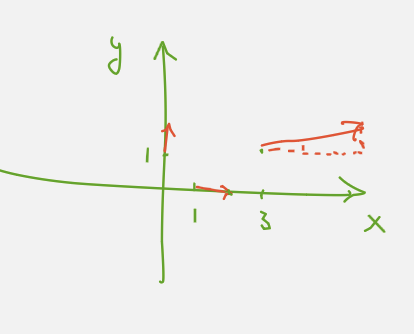
\includegraphics[width=.3\textwidth]{grad.png} 
\end{center}
Векторные линии:
\begin{equation*}
    y' = \frac{y}{x}\ \ \dv{y}{x}= \frac{y}{x}\ \ \frac{dy}{y}= \frac{dx}{x}\ \ \int\frac{dy}{y} = \int\frac{dx}{x}
\end{equation*}
\begin{equation*}
    ln|y| = ln|x| + C;\ C = ln|C_1|
\end{equation*}
\begin{equation*}
    |y|= |C_1x|
\end{equation*}
\begin{equation*}
    y= C_1x,\ C_1\in \mathbb{R}
\end{equation*}
\begin{center}
    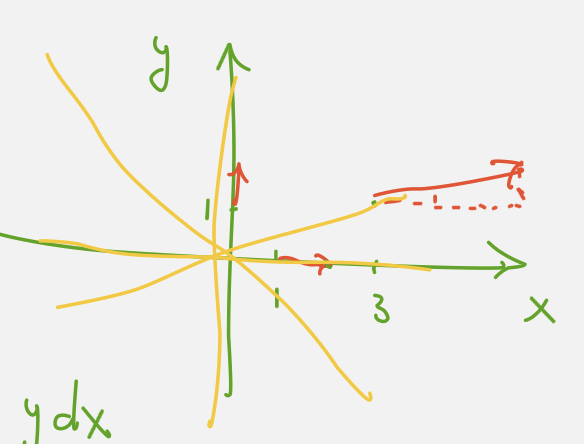
\includegraphics[width=.3\textwidth]{ans_grad.png} 
\end{center}
Свойства градиента:\\
1) Градиент скалярной функции z(x;y) каждой точке направлен перпендикулярно к линии уровня z(x;y), проходящей через эту точку.

Доказательство:

\begin{equation*}
    z = z(x;y)\ \ z(x;y) = C - level\ line
\end{equation*}
\begin{equation*}
    k_1 = y' = -\frac{z'_x}{z'_y} - \text{угловой коэфицент касательной к линии уровня}
\end{equation*}
\begin{equation*}
    grad\ z(x;y) = (z'_x; z'_y)
\end{equation*}
\begin{equation*}
    k_2 = \frac{z'_y}{z'_x}
\end{equation*}
\begin{equation*}
    k_1\cdot k_2 = -\frac{z'_x}{z'_y}\cdot \frac{z'_y}{z'_x} = -1
\end{equation*}

2)Линейность
\begin{equation*}
    grad(f+g) = grad(f)+ grad(g)
\end{equation*}
\begin{equation*}
    grad(\alpha f)  =\alpha grad(f), \alpha\cdot\in \mathbb{R}
\end{equation*}
3)
\begin{equation*}
    grad(f\cdot g) = f\cdot grad(g) + g\cdot grad(f)
\end{equation*}
4)
\begin{equation*}
    \pdv{z}{l}= \text{проекция grad(z)}
\end{equation*}
Докажем
\begin{equation*}
    \pdv{z}{l}= \pdv{z}{x}cos\alpha+\pdv{z}{y}cos\beta = (\pdv{z}{x}; \pdv{z}{y})\cdot (cos\alpha;cos\beta) = gradz\cdot \overline{l}^o = |grad\ z|\cdot |\overline{l}^o|\cdot cos\phi = |grad\ z|\cdot \phi 
\end{equation*}
\begin{equation*}
    \phi = \angle (grad\ z; \overline{l}^o)
\end{equation*}
По какой траектории движется точка P при изменении направления $\overline{l}$?
\begin{center}
    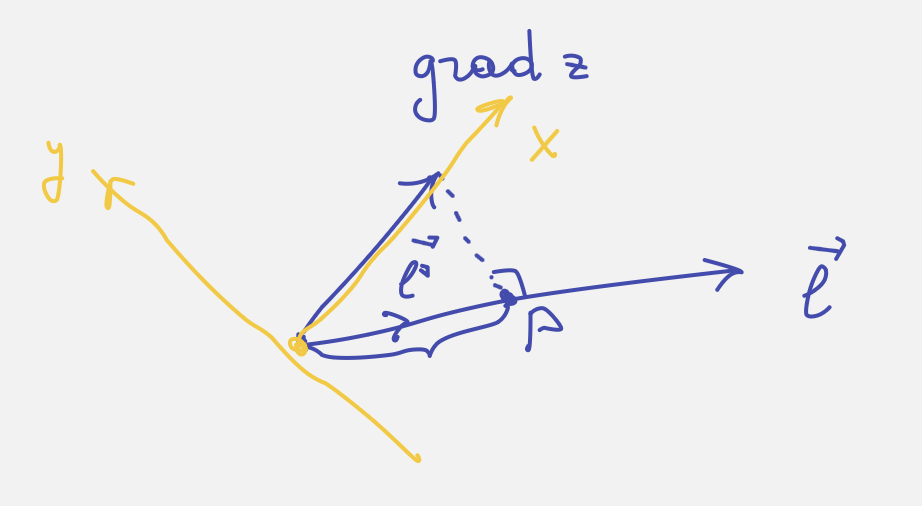
\includegraphics[width=.3\textwidth]{gradx.png}
\end{center}
P = (x;y) - точка
\begin{equation*}
    x = \pdv{z}{l}\cdot \cos\phi
\end{equation*}
\begin{equation*}
    y = \pdv{z}{l}\cdot \sin\phi
\end{equation*}
\begin{equation*}
    \pdv{z}{l} = |grad\ z|\cdot \cos\phi
\end{equation*}
\begin{equation*}
\begin{cases}

        x = |grad\ z|\cdot \cos^2\phi\\

        y = |grad\ z|\cdot \cos\phi \sin\phi

\end{cases}->\ 
\begin{cases}

    x = \frac{1}{2}|grad\ z|\cdot (1+cos2\phi)\\

    y = |grad\ z|\cdot \sin2\phi

\end{cases}->\ 
\begin{cases}

    (x-\frac{|g|}{2})^2 = (\frac{1}{2}|g|\cdot cos2\phi)^2\\

    y^2 = (\frac{1}{2}|grad\ z|\cdot \sin2\phi)^2

\end{cases}
\end{equation*}

\begin{equation*}
    \left(x - \frac{|g|}{2}\right)^2+y^2 = \frac{|g|^2}{4}
\end{equation*}
окружность с центром в $(\frac{|g|}{2};0)\ and R = \frac{|g|}{2}$ 

доказано
5) 
\begin{equation*}
    \pdv{z}{l}, \ \overline{l} = grad(z),\ = maximum
\end{equation*}
6)
\begin{equation*}
    \pdv{z}{l}, \ \overline{l} \bot  grad(z),\  = 0
\end{equation*}
\textbf{Example}

Найти наибольшую крутизну(угол наклона поверхности) подъёма поверхности

\begin{equation*}
    z = ln(x^2+2y^2) \ \ in\ \  M(6;4\sqrt{2};ln(100))
\end{equation*}
\begin{equation*}
    \pdv{z}{l} = |grad\ z| = tg\ \alpha
\end{equation*}
\begin{equation*}
    |grad\ z| = (\frac{2x}{x^2+2y^2}; \frac{4y}{x^2+2y^2})
\end{equation*}
\begin{equation*}
    grad\ z(M) = (\frac{12}{100};\frac{16\sqrt{2}}{100})
\end{equation*}
\begin{equation*}
    |grad\ z(M)| \approx  \frac{1}{4} = tg\alpha
\end{equation*}
\section{Касательная прямая и нормальная плоскость кривой}
L - кривая на плоскости R 2х мер


1)Явно:
\begin{equation*}
    y = y(x)\ \ x\in [a;b]
\end{equation*}
Example:
\begin{equation*}
    L:\ y=x^2
\end{equation*}
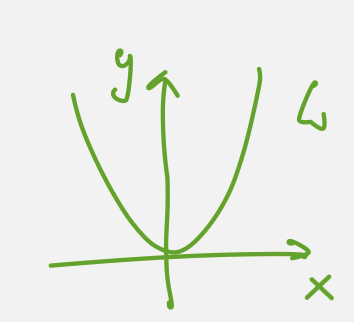
\includegraphics[width=.3\textwidth]{yavno.png} 

2)Неявно:
\begin{equation*}
    L:\ F(x,y) = 0
\end{equation*}
Example:
\begin{equation*}
    L:\ y=x^2
\end{equation*}
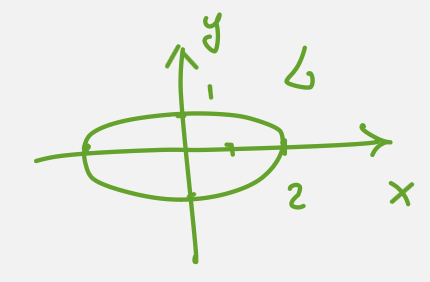
\includegraphics[width=.3\textwidth]{neyavno.png} 

3)Векторно:
\begin{equation*}
    L:\ \overline{r} = \overline{r}(t)
\end{equation*}
\begin{equation*}
    \begin{cases}
        x = x(t)\\
        y = y(t)
    \end{cases}
\end{equation*}
Example:
\begin{equation*}
    \begin{cases}
        x = 2cos(t)\\
        y = sin(t)
    \end{cases}
    \ \ t\in [0;2\pi)
\end{equation*}
\\ \\
L - кривая в пространстве R 3х мер

1)
\begin{equation*}
    L: \overline{r} = \overline{r}(t)
\end{equation*}
\begin{equation*}
    \begin{cases}
        x = x(t)\\
        y=y(t)\\
        z=z(t)
    \end{cases}
    \ \ t\in [\alpha;\beta]
\end{equation*}
Example:
\begin{equation*}
    \begin{cases}
        x = 2cos(t)\\
        y=sin(t)\\
        z=t
    \end{cases}
    \ \ t\in [0;2\pi)
\end{equation*}
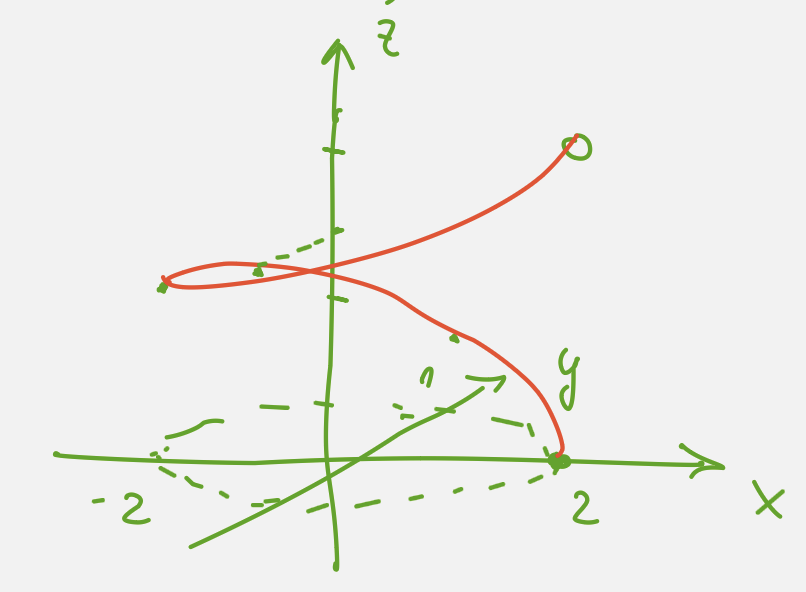
\includegraphics[width=.3\textwidth]{spiral.png} 

2)Задано неявно, как пересечение двух плоскостей
\begin{equation*}
    \begin{cases}
        F_1(x,y,z) = 0\\
        F_2(x,y,z) = 0
    \end{cases}
\end{equation*}
Example:
\begin{equation*}
    \begin{cases}
        x^2+y^2+z^2=4\\
        x^2+y^2=2y
    \end{cases}
\end{equation*}
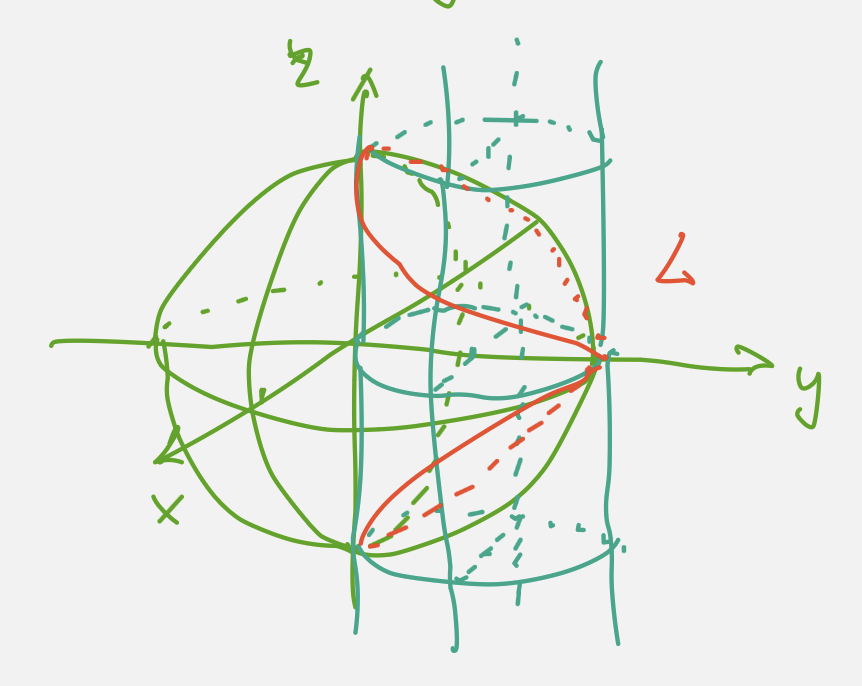
\includegraphics[width=.3\textwidth]{neyavno2.png} 
\\ \\
1) 
\begin{equation*}
    \begin{cases}
        x = x(t)\\
        y=y(t)\\
        z=z(t)
    \end{cases}
    \ \ \overline{r} = \overline{r}(t)
\end{equation*}
\begin{equation*}
    \overline{\tau} = \frac{d\overline{r}}{dt} = \lim_{\Delta t->0}\frac{\Delta \overline{r}(t)}{\Delta t} = \frac{dx}{dt}\overline{i}+\frac{dy}{dt}\overline{j}+\frac{dz}{dt}\overline{k} = (x'(t); y'(t); z'(t))
\end{equation*}
при
\begin{equation*}
    x(t),\ y(t),\ z(t)\ - \text{гладкая кривая}
\end{equation*}
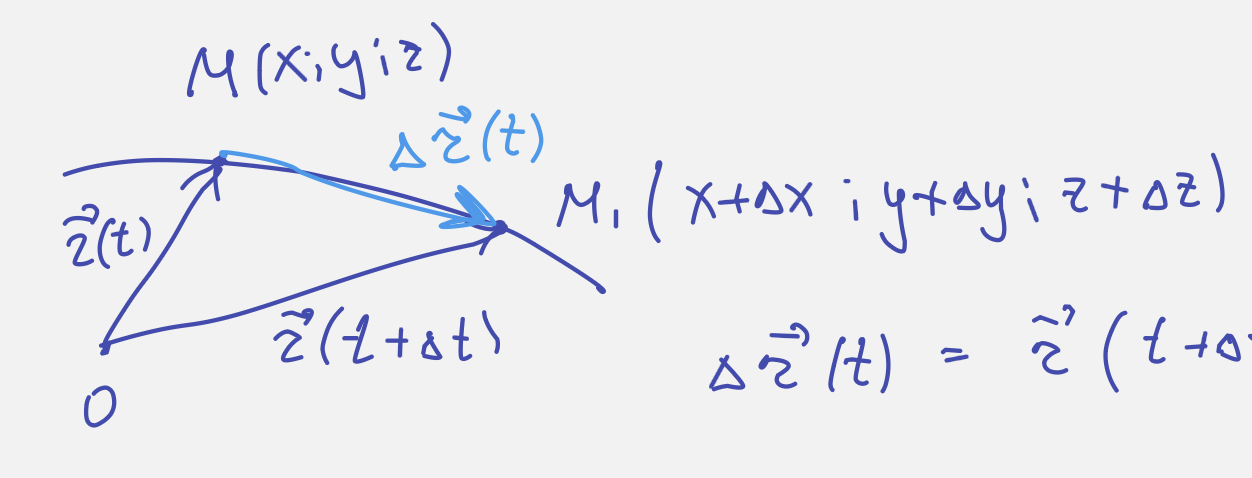
\includegraphics[width=.3\textwidth]{kas}
\begin{equation*}
    \Delta \overline{r}(t)= \overline{r}(t+\Delta t) - \overline{r}(t)
\end{equation*}
Уравнение касательной прямой в точке кривой:
\begin{equation*}
    \frac{x-x_0}{a} = \frac{y-y_0}{b} = \frac{z-z_0}{c}
\end{equation*}
\begin{equation*}
    M_0(x_0;y_0;z_0), \ \overline{s}(a;b;c)
\end{equation*}
=>
Уравнение касательной
\begin{equation*}
    \frac{x-x_0}{x'(t_0)} = \frac{y-y_0}{y'(t_0)} = \frac{z-z_0}{z'(t_0)} \ \ M_0:
    \begin{cases}
        x_0 = x(t_0)\\
        y_0=y(t_0)\\
        z_0=z(t_0)
    \end{cases}
\end{equation*}
\\ \\
Уравнение нормальной плоскости в точке кривой
\begin{equation*}
    A(x-x_0)+B(y-y_0)+C(z-z_0) = 0;\ \overline{n}(A;B;C);\ M_0(x_0;y_0;z_0)
\end{equation*}
=>
\begin{equation*}
    x'(t_0)(x-x_0)+y'(t_0)(y-y_0)+z'(t_0)(z-z_0) = 0
\end{equation*}
\section{Касательная плоскость и нормальная прямая поверхность}
Г- поверхность в пространстве R 3х мер

1) Явное
\begin{equation*}
    G:\ z = f(x;y);\ x = g(z;y);\ y = h(x;z);\ 
\end{equation*}
Example:
\begin{equation*}
    y = x^2 +z^2 
\end{equation*}
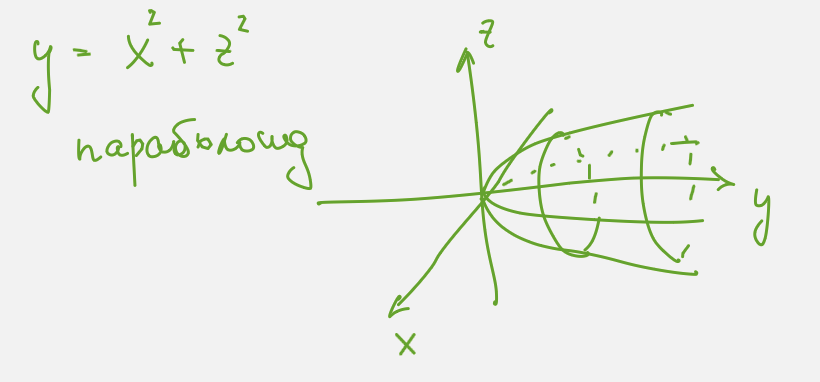
\includegraphics[width=.3\textwidth]{parabol.png}

2) Неявное
\begin{equation*}
    G:\ F(x;y;z)=0\ 
\end{equation*} 
Example:
\begin{equation*}
    x^2-y^2+z^2-1=0
\end{equation*}
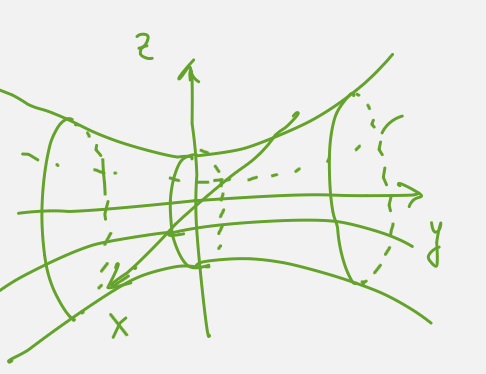
\includegraphics[width=.3\textwidth]{parabalobel.png} 

3) Параметрически
\begin{equation*}
    \begin{cases}
        x = x(u;v)\\
        y = y(u;v)\\
        z = z(u;v)
    \end{cases}
\end{equation*}
Векторное:
\begin{equation*}
    \overline{r} = \overline{r}(u;v)
\end{equation*}
Example:
\begin{equation*}
    x = 2\cos\phi\sin\theta 
\end{equation*}
\begin{equation*}
    y = 2\sin\phi\sin\theta 
\end{equation*}
\begin{equation*}
    z = 2\cos\theta 
\end{equation*}
$\phi$ - азимутальный угол\\
$\theta$ - зенитный угол\\
$\phi \in [0;2\pi]$\\
$\theta \in [0;\pi]$\\
\begin{equation*}
    \measuredangle x^2+y^2+z^2 = 4cos^2\phi sin^2\theta+4sin^2\phi sin^2\theta + 4 cos^2\theta = 4sin^2\theta +4cos^2\theta = 4
\end{equation*}
\begin{equation*}
    x^2+y^2+z^2 = 4
\end{equation*}
сфера с центром в точке (0;0;0) и R=2\\
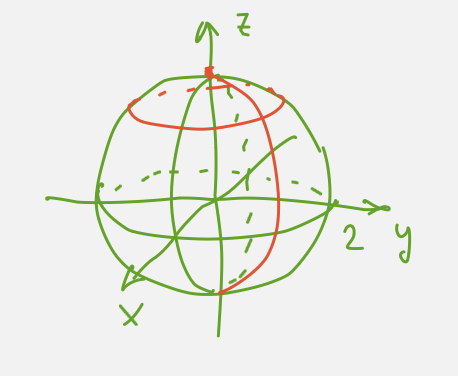
\includegraphics[width=.3\textwidth]{sphere.png}
\\ \\
Касательная к поверхности в точке - это касательная к кривой на поверхности, проходящей через эту точку.
\begin{equation*}
    G:\ F(x;y;z) = 0;\ \ P(x;y;z) - point
\end{equation*}
P - обыкновенная точка к поверхности, если в этой точке все чатные производные $\pdv{F}{x}, \pdv{F}{y}, \pdv{F}{z} $ этой поверхности - существуют, непрерывны и не все =0
\\
P - особая, если все производные ранвы ноль или одно из них не существует.
\\ \\
Example
\begin{equation*}
    F(x,y,z) = x^2+y^2-z^2 = 0\ (cono)
\end{equation*}
\begin{equation*}
    \pdv{F}{x} = 2x;\  \pdv{F}{y}= 2y;\ \pdv{F}{z}= -2z;\ \ \ \ => P(0,0,0)
\end{equation*}

Theorem  - о касательной плоскости 
\begin{equation*}
    P - \text{ обыкновенная точка =>}\ in\ P \text{ все касательные лежат в одной плоскости}
\end{equation*}
Доказательство
\begin{equation*}
    L:\ 
    \begin{cases}
        x = x(t)\\
        y = y(t)\\
        z = z(t)
    \end{cases} \ \ \ \ 
    \overline{\tau} = (x'(t), y'(t), z'(t))
\end{equation*}
\begin{equation*}
    G: F(x;y;z) = 0
\end{equation*}
т.к. точки L лежат на поверхности, то 
\begin{equation*}
    F(x(t), y(t), z(t)) = 0\ \ \ | \cdot \frac{d}{dt}
\end{equation*}
\begin{equation*}
    \pdv{F}{x}\cdot \pdv{x}{t} + \pdv{F}{y}\cdot \pdv{y}{t} + \pdv{F}{z}\cdot \pdv{z}{t} = 0
\end{equation*}
\begin{equation*}
    grad(F)\cdot \overline{\tau} = 0
\end{equation*}
\begin{equation*}
    grad(F) - \text{ вектор нормали n}
\end{equation*}
\begin{equation*}
    \forall \overline{\tau} \perp grad(\overline{F}(P))
\end{equation*}
все касательные лежат в одной плоскости 

доказано
\\  \\
Касательная плоскость:
\begin{equation*}
    \pdv{F}{x}\left(P\right)(x-x_0)+\pdv{F}{y}\left(P\right)(y - y_0) +\pdv{F}{z}\left(P\right)(z - z_0) = 0; \ \ \  P(x_0;y_0;z_0)
\end{equation*}
Нормальная прямая:
\begin{equation*}
    \frac{x-x_0}{\pdv{F}{x}\left(P\right)} = \frac{y-y_0}{\pdv{F}{y}\left(P\right)} = \frac{z-z_0}{\pdv{F}{z}\left(P\right)}
\end{equation*}

\section{Полярные координаты}
$\phi$ - полярный угол 

$\rho$ - полярный угол

\begin{equation*}
    \begin{cases}
        \rho \geq 0 \\
        0\leq \phi < 2\pi
    \end{cases}
    \begin{cases}
        x=\rho\cdot \cos \phi\\
        y = \rho \sin \phi
    \end{cases}
\end{equation*}
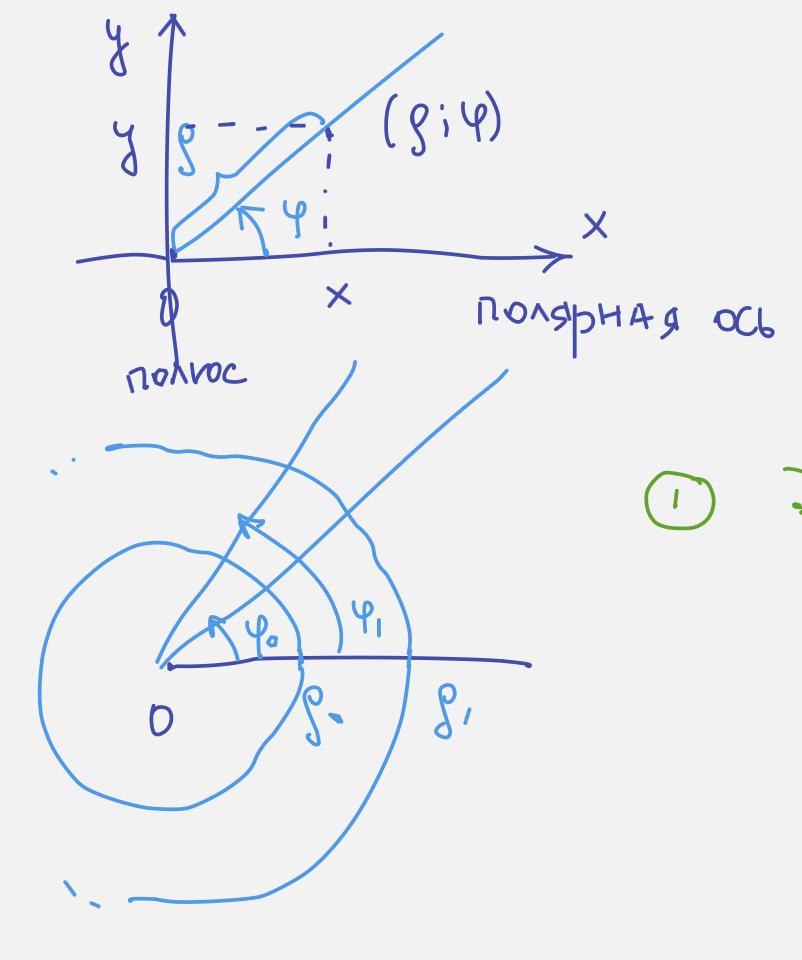
\includegraphics[width=.3\textwidth]{psk} 

\section{Цилиндрические и сферические координаты}
\begin{minipage}{.5\textwidth}
Цилиндрическая

z - ось апликат\\
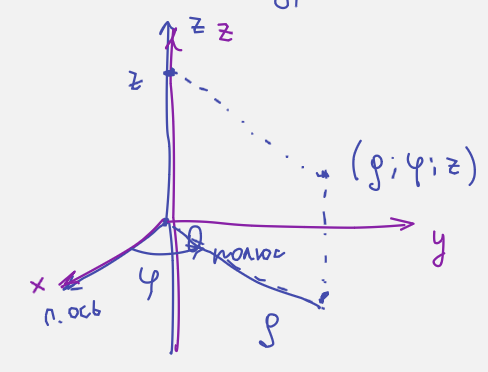
\includegraphics[width=.6\textwidth]{chill}\\
\begin{equation*}
    \rho \geq 0;\ 0\leq\phi<2\pi;\ z\in \mathbb{R}
\end{equation*}
\begin{equation*}
    \begin{cases}
        x= \rho cos\phi\\
        y = \rho sin\phi\\
        z=z
    \end{cases}
\end{equation*}
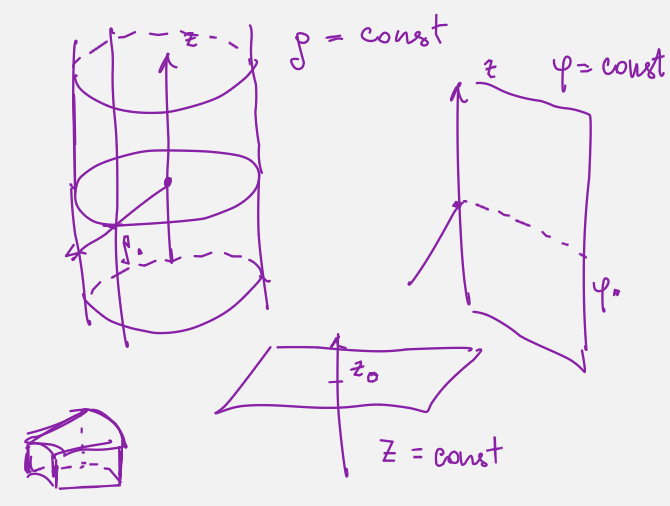
\includegraphics[width=.6\textwidth]{CHILLCONST.png}\\
\end{minipage}
\hfill
\begin{minipage}{.5\textwidth}
Сферическая

$\phi$ - азимутальный 

$\theta$ - зенитный угол

$r$ - расстояние\\
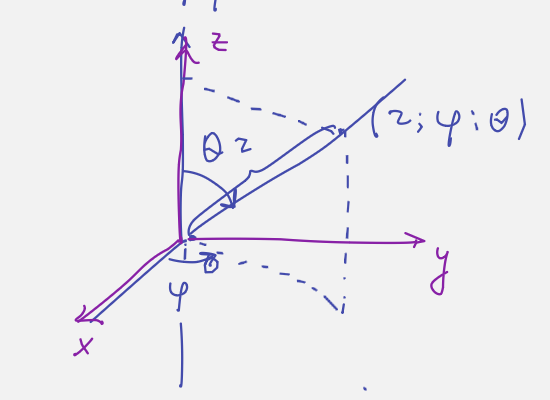
\includegraphics[width=.6\textwidth]{sphere12.png} 
\begin{equation*}
    r \geq 0;\ 0\leq \phi<2\pi;\ 0\leq \theta \leq \pi
\end{equation*}
\begin{equation*}
    \begin{cases}
        x= r\cdot \sin\phi\cos\theta\\
        y = r\cdot \sin\phi \sin\theta\\
        z=r\cdot \cos\theta
    \end{cases}
\end{equation*}
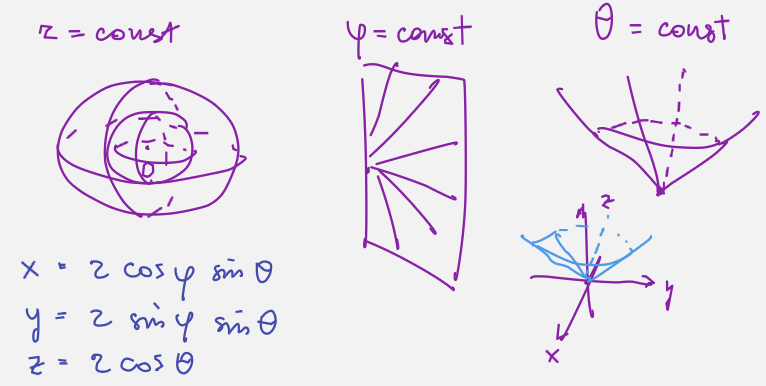
\includegraphics[width=.6\textwidth]{sphereconst.png} 
\end{minipage}
% 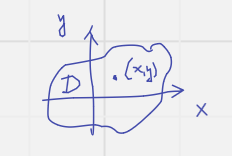
\includegraphics[width=.3\textwidth]{1.1} 
\end{document}
